\section{Outils mis en place}

Afin de mener à bien notre projet, nous avons utilisé différents outils de gestion de projets :

\begin{itemize}
	\item Pour permettre le suivi du projet, nous avons mis en ligne un site web, ce dernier utilise le CMS Wordpress : \url{http://www.ecole.ensicaen.fr/~lvimont/}

		\begin{figure}[h!]
			\centering
			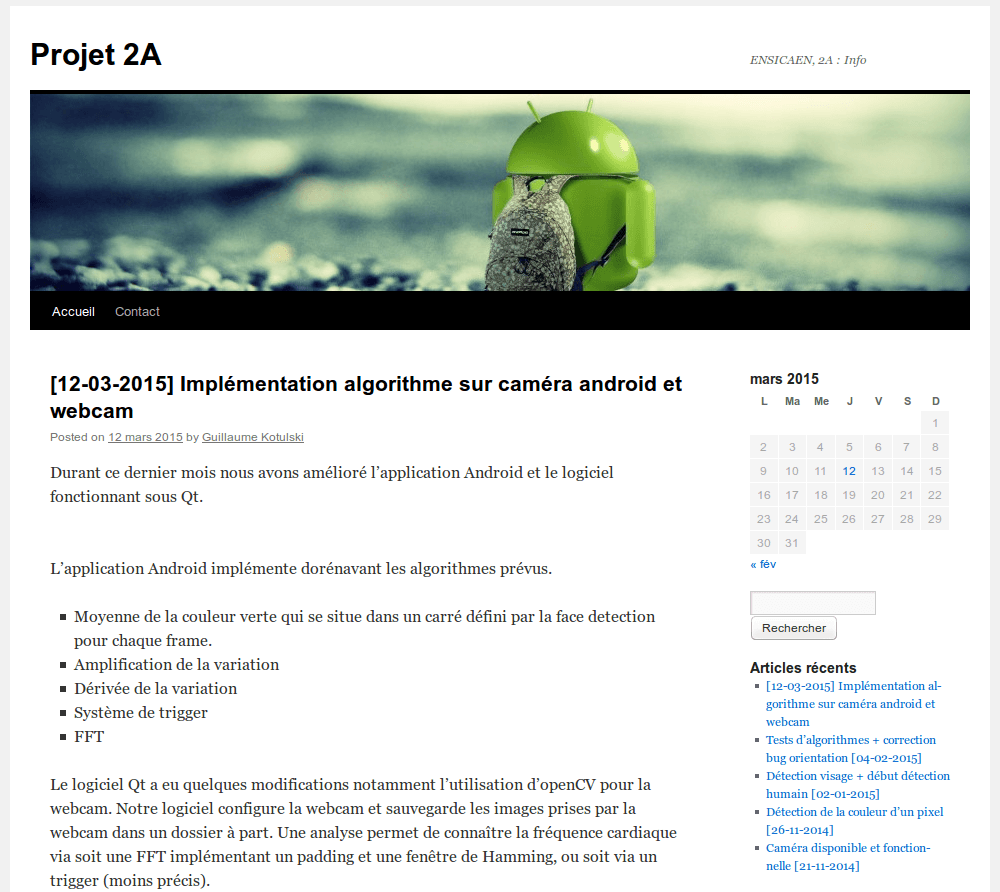
\includegraphics[width=0.9\textwidth]{data/website.png}
			\caption{Capture d'écran du site web.}
		\end{figure}

	\item Afin de partager le code source entre nous, nous avons utilisé le gestionnaire de versions Git :
		\begin{itemize}[label=\textbullet]
			\item Application Android: \url{https://github.com/F4r3n/Vamp}
			\item Logiciel de traitement d'images: \url{https://github.com/F4r3n/ImageProject.git}
		\end{itemize}
	\item Enfin, pour pouvoir avoir une vue globale sur les tâches à réalisées, en cours et déjà faites, nous avons utilisé le gestionnaire de projets Trello.
\end{itemize}

\section{Technologies utilisées}

\begin{itemize}[label=\textbullet]
	\item Qt : Nous avons utilisé la librairie Qt pour pouvoir créer notre application qui permettait de tester les algorithmes.
	\item Android : La programmation sous Android s'est faite en utilisant le Java et de l'XML.
	\item OpenCV : Utilisation de la webcam et application utilisant la caméra gérée par OpenCV
	\item Python : Traitement des données pour création d'un graphique et permet une meilleure vérification des résultats
\end{itemize}

\section{Algorithme mis en place}

L’\oe il humain est limité, en effet il est incapable de voir les subtils changements temporels. Alors qu'au contraire en effectuant des traitements sur une vidéo, on est capable de
 révéler ces changements comme par exemple, la circulation du sang. Le sang parcourt notre corps de haut en bas de manière perpetuelle, ce mouvement imperceptible pour un oeil humain peut
 être capturée par notre téléphone portable. En travaillant sur ces infimes changements, on peut même grâce à ça réussir à connaître le pouls d'une personne. Mais comment obtenir ces*
  changements ? Comment savoir où se situe le visage ?\\

Dans un premier temps, nous devons arriver à détecter la présence d'un visage humain devant l'appareil, en utilisant l'api de Google et même la libraire d'OpenCV, cela se fait bien.
Grâce à cette détection, nous pouvons obtenir les coordonnées du visage détéctées.\\

Maintenant que nous savons où se situe le visage, nous nous demandons comment reconnaître une fréquence ?\\

 \subsection{Choix de l'espace de couleur}
 Le choix de l'espace de couleur est primordial. C'est en fonction de celui-ci que nous obtiendrons des résultats cohérents ou non.\\
 Un des points important à prendre en compte fut le changement de luminosité, en se placant dans les espaces HSV, HSL ou YUV et en ne sélectionnant que les canaux Hue et Saturation par exemple pour HSV. Nous
  pensions obtenir des résultats ne dépendant pas de la luminosité. Sauf que les résultats obtenus par ces espaces de couleur n'étaient pas cohérents.\\
 \\
 Le second espace de couleur choisit fut RGB, en effet même si celui-ci dépend fortement de la luminosité, nos résultats étaient meilleurs. Nous pouvions visualiser plus efficacement les changements de
 variation avec une dérivée.\\
 \\
 Après le choix de cet espace de couleur nous devions voir quel canal permetterait d'obtenir des variations les plus fortes. Pour ce faire nous avons visualisé les résultats de notre algorithme sur des personnes ayant des couleurs de peau différentes et avec les différents canaux (Red, Green, Blue). Nous remarquions que les résultats étaient meilleurs si nous utilisions seulement le canal Green.


 \subsection{Obtention des données}
 Nous avons donc fait une moyenne du canal vert (c'est le canal vert qui varie le plus) pour chaque pixel se situant dans un rectangle (en l’occurrence le rectangle délimitant le visage).
 Et ceci pour chaque frame que l'on capturait, nous obtenions une certaine valeur.
 Après obtention de ces valeurs, nous pouvions les traiter.
 La variation des valeurs étant très grande, nous avons dans un premier temps fait une moyenne glissante. Puis, pour amplifier les variations nous avons avons fait une dérivée de Taylor.
 Nos valeurs étant prêtes à être analysées, nous les avons traitées de deux façons différentes.
 La première, la plus simple fut le Trigger, qui nous permettait d'avoir une fourchette de pulsation.\\ La deuxième plus longue, une FFT, nécessitait des étapes de calcul supplémentaires telles qu'un fenêtrage de Hamming ou encore un padding, mais donnait des résultats plus précis.
 \\
 Ces deux analyses nous ont permis d'avoir le pouls de notre utilisateur (dans le cas idéal, c'est à dire lorsque la caméra et l'utilisateur ne bougeaient presque pas).
 \\

Nous avons remarqué que la collecte des données n'accentuait pas assez les variations, nous avons donc créé une deuxième méthode qui en restant basé sur le même principe que la première technique, nous découpions notre image
par zone de petits carrés de pixels. Par exemple une zone serait d'une taille de 5*5. On réalise ainsi une moyenne de chaque zone, puis par la suite une moyenne de ces moyennes. Enfin on rapplique les mêmes fonctions citées précédemment.

\begin{figure}[h!]
	\centering
	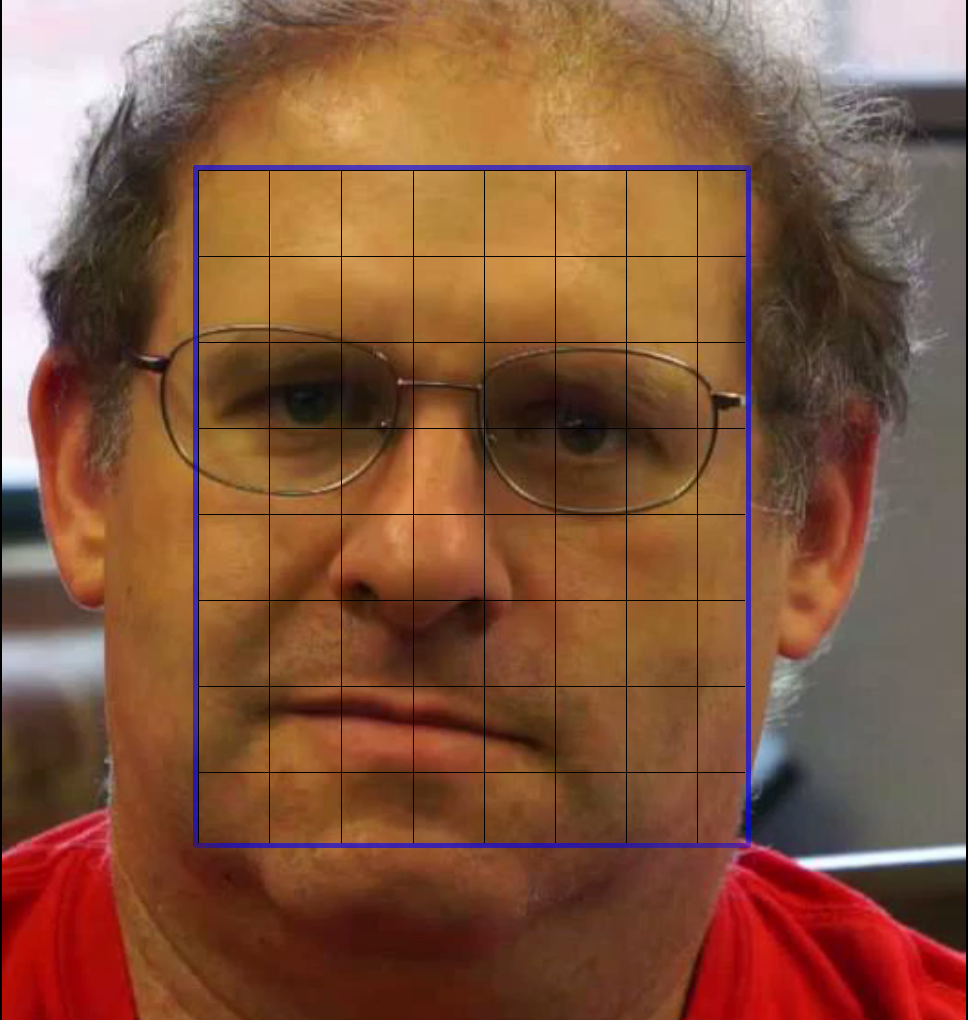
\includegraphics[width=0.5\textwidth]{data/algo-schema.png}
	\caption{Schéma de l'algo précédent}
\end{figure}


\section{Solutions mis en place}

Durant le projet nous avons développé plusieurs outils pour répondre au besoin. Une application Android qui permettrait d'utiliser le moyen d'authentification désiré et ainsi déverrouiller le smartphone d'une
personne. Un logiciel C++ utilisant la librairie Qt a également été mis en place, afin de pouvoir tester plus facilement les algorithmes que nous voulions développer. Dans la suite du projet, il a également
permis d'utiliser la webcam.

\subsection{Développement Android}

Notre application Android est capable d'utiliser la caméra frontale de n'importe quel smartphone. L'api d'Android propose une classe appelée FaceDetectionListener qui va permettre de
 capter, les visages présent devant une caméra, grâce à ce système il est possible de dessiner un Rect (c'est à dire un rectangle) autour du visage de la personne. C'est notre classe
  DisplayedFace qui se charge de ce travail.
Une fois la reconnaissance mis en place, nous avons utilisé la fonction
\href{http://developer.android.com/reference/android/hardware/Camera.PreviewCallback.html#onPreviewFrame\%28byte\%5B\%5D,\%20android.hardware.Camera\%29}{onPreviewFrame}. Cette dernière permet d'enregistrer
en temps réel, les données. On lance un compteur quand la première reconnaissance d'un visage a lieu, ce dernier va durer 5 secondes.\\

\begin{figure}[h!]
	\centering
	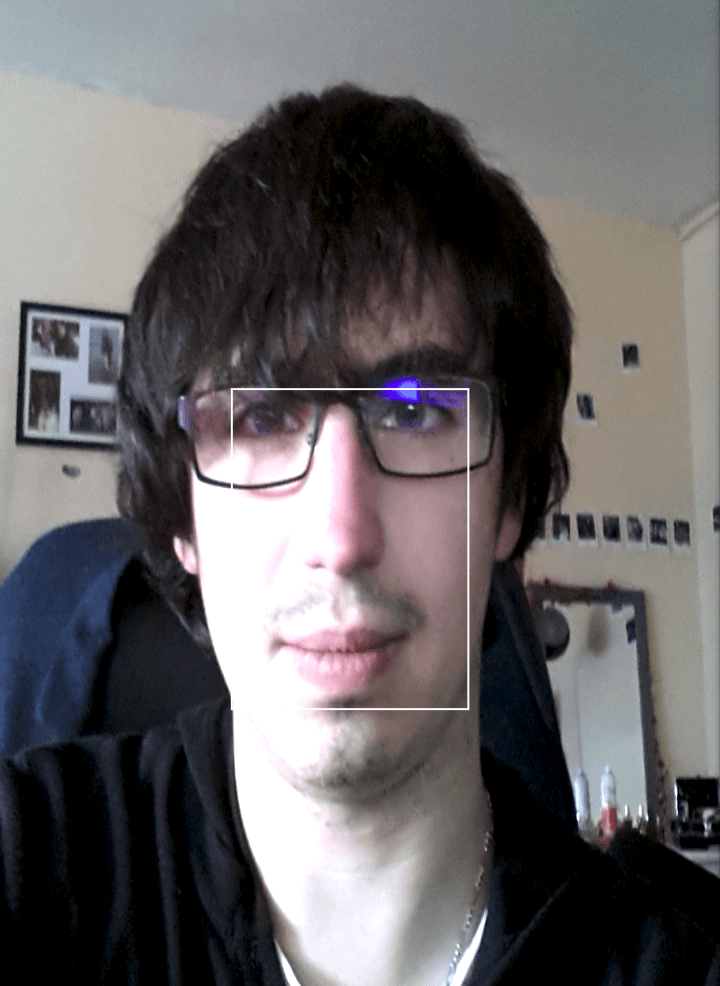
\includegraphics[width=0.5\textwidth]{data/appAndroid.png}
	\caption{Aperçu de l'application Android}
\end{figure}

Les données ainsi récoltées sont au format de l'espace de couleur \href{http://fr.wikipedia.org/wiki/YUV}{YUV}. Nous devons donc convertir ces données au format RGB qui se révèle plus évocateur au niveau des variations.

A la fin du compteur, on réalise une dérivée, puis une amplification des valeurs obtenues. On observe alors les variations qu'on obtient et on conclut alors sur la présence ou non d'un humain.\\
\\
L'api de Google est très rapide pour détecter un visage et pour nous fournir ces coordonnées en faisant très peu de calculs. Mais celle-ci ne suit pas les petits changements de position, par exemple lorsque l'utilisateur prend une vidéo il bouge légèrement ce qui peut changer le résultat final.\\
\\
Pour résoudre ce manque nous avons codé une application fonctionnant avec OpenCV, celle-ci suit parfaitement le visage lorsqu'il bouge. Mais le temps de traitement d'une image par OpenCV est beaucoup plus lent que l'api de Google. Nous tournons à environ 7 FPS en utilisant la back-caméra et 2 FPS en utilisant la front-caméra, ce qui n'est pas idéal.
\begin{figure}[h!]
	\centering
	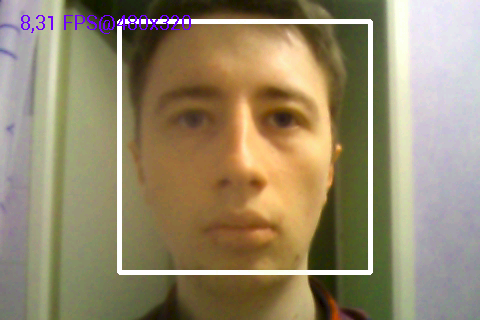
\includegraphics[width=0.8\textwidth]{data/opencv.png}
	\caption{Aperçu de l'application OpenCV}
\end{figure}
\\
\\
L'application sous OpenCV permet de faire une FFT et un système de Trigger, en croisant les résultats donnés par ces deux systèmes nous obtenons un meilleur résultat que s'il n'y avait que le Trigger.

\subsection{Développement C++}

Nous avons créé un logiciel C++ nous permettant de tester nos algorithmes avant de les implémenter sous Android.
Ce logiciel a de nombreuses fonctionnalités, notamment le découpage d'une vidéo en images pour permettre une analyse plus poussée.
Nous utilisons Avconv qui permet de découper une vidéo de n'importe quelle taille en une multitude d'images. (15 images * taille de la vidéo)
Après avoir découpé la vidéo en images nous faisons une analyse sur ces images.
Cette analyse se découpe en plusieurs étapes.\\

Dans un premier temps nous dessinons un rectangle autour d'un visage (si la fonction du rectangle automatique n'est pas enclenchée).
Puis nous choisissons le type d'analyse à effectuer, il y en a deux types:\\
\begin{itemize}
	\item L'une fait la moyenne de tous les pixels qui se situe dans le carré
	\item La seconde découpe le rectangle en plusieurs zones de 5*5 puis amplifie les variations et fait une moyenne des valeurs
\end{itemize}
Après avoir lancé l'analyse, nous affichons les courbes ainsi obtenues par notre application.\\

Nous pouvons voir la FFT, l'amplification, la dérivée ou une combinaison de plusieurs méthodes.
L'amplification utilise la dérivée de Taylor du premier degré.
La FFT utilise un filtre passe-bas combiné avec une fenêtre de Hamming et un padding.
La FFT permet de connaître le rythme cardiaque d'une personne de manière précise si l'image est assez stable.
Nous avons créé un Trigger qui permet aussi de connaître la fréquence cardiaque d'une personne, mais de manière moins précise, le Trigger nous donne une fourchette de valeurs.\\

Si l'espace de couleur que nous avons choisi ne donne pas des résultats corrects nous pouvons en choisir un autre.
Nous avons différents espaces de couleur disponibles dont RGB, HSL, HUV et nous pouvons lancer une analyse avec un espace de couleur différent de RGB.\\

Les analyses avec des vidéos classiques n'étant pas suffisantes pour nos tests, nous avons dû faire une analyse avec des vidéos de la webcam.
La webcam est configurée et lancée via la librairie OpenCV et nous enregistrons les images de la webcam avec une fréquence de 15 frames pas seconde.\\

\section{Problèmes rencontrés}

\subsection{Limitation des sessions à l'ENSICAEN}

Lors du projet, nous avons rencontré de nombreux problèmes. L'un des plus embêtants fut la limite des sessions à l'Ensicaen. En effet, nos sessions disposent d'une taille limitée, nous
 pouvons uniquement travailler sous Windows (car c'est seulement sous cet environnement que sont installés les outils Android) hors nous disposons d'uniquement 150 Mo, or rien qu'avec
  Firefox, si nous ne nettoyons pas régulièrement l'historique, la session se retrouve complète. Nous avons malheureusement expérimenté le souci et perdu ainsi, une après-midi de travail.

\subsection{Problèmes rencontrés lors du développement Android}

Nous avons eu un problème de rotation, les coordonnées que l'on converser se révélaient mauvaise. Afin d'éviter cela, nous avons décidé de forcer le mode portrait.

La première version de notre application était capable d'enregistrer 15 frames par seconde, or au final on obtenait seulement une trentaine de valeurs, cela était dû à la conversion du
 format YUV au format RGB que l'on effectuer à chaque fois que nous rentrons dans la fonction onPreviewFrame, comme la conversion est coûteuse O(n\up{2}), on perdait des valeurs. Pour
  optimiser, le nombre de valeurs nous effectuons maintenant la conversion une fois le timer fini. On réalise alors dans la boucle une simple sauvegarde des données brutes.
Toutefois cette méthode, nous a causé pas mal de soucis, notamment des out of memory, c'est-à-dire, que nous réalisions une allocation trop grande par rapport à la mémoire disponible
\ldots{}\\
\\
Même si l'algorithme fonctionnait avec des vidéos, ceci ne voulait pas dire qu'il fonctionnerait sous Android. En effet lorsque avec la caméra on se prend en vidéo on bouge légèrement,
ce qui pose de nombreux problèmes de stabilité. Les variations que nous obtenons alors ne seraient plus celle de la pulsation mais celles du mouvement régulier de la main.
